%\textbf{What we have to work with: topics, features, feature attributes}
In this section, we analyze the informativeness of our defined features in Sec~\ref{sec:datasetStatistics} and the effect of their attributes on learning targeted topical social sensor. To this end, the goal is to answer the following questions in this section.

\begin{itemize}
\item What are the best features for learning social sensors and do they differ by topic?
\item For each feature type, do any attributes correlate with importance?
\end{itemize}

To answer these questions, we use Mutual Information as the metric for evaluating features. Mutual Information is a general method for measuring informativeness, which is a measure of amount of information one random variable contains about another random variable. In order to calculate amount of information that a feature $d_{i} \in \{from, hashtag, mention, term, location\}$ provides w.r.t topic $t \in \{NaturalDisaster, Epidemics, ...\}$, mutual information is defined as:

\begin{multline}
I(t, f_k)= \\
 \sum_{t \in \{ true, false \}} \sum_{f_k\in \{ true, false\}}p(f_k,t)\log \left ( \frac{p(f_k,t)}{p(f_k)p(t)} \right )
 \label{eq:eq1}
\end{multline}

Where higher values for this metric indicate more informative features for the specified topic.

In order to answer the first question on what are the best features for learning social sensors, we provide mean of Mutual Information values for each feature across different topics in Table ~\ref{fig:avgMI}. The last column in Table ~\ref{fig:avgMI} shows the average of mean Mutual Information for the feature. From analysis of Table ~\ref{fig:avgMI}, we can make a set of observations:

\begin{itemize}
\item The \textit{Term} and \textit{Location} features are the most prevalent features.% and in general, the more features you have, the better the chance that one is useful.
\item There are a few topics such as \textit{IranDeal} and \textit{tennis}, that are less sensitive to the selection of a specific set of features and are in the list of top $4$ MAP scores of \textit{Logistic Regression}.%providing evidence on the power of learning social sensors for these cases.
\item The Location feature provides more information regarding \textit{HumanDisaster}, \textit{LBGT}, and \textit{Soccer} topics.
\item Sorting features based on their average mean values across different topics results in the following order for informativeness measure of features: \textit{Term}, \textit{Location}, \textit{Hashtag}, \textit{Mention}, \textit{From}.
\end{itemize}

In general, this presents evidence on the need for learning the weights of features for each topic as there is no specific selection of features that would separate various topics from each other.

Also, in order to show the power of Mutual Information metric, we present the top $5$ features for each topic in Table~\ref{table:top10MItopicsLocations}. It can be observed that the different locations, hashtags, or terms shown as the top features based on Mutual Information are actually in relation with the specific topic.

%%%%%%%%%%%%%%%%%%%%%%%%%%%%%%%%%%%%%%%%%%%%%%%%%%%%%%%%%%%%%%%%%%%%%%%%%%%
%\begin{figure}[h!]
%\centering
%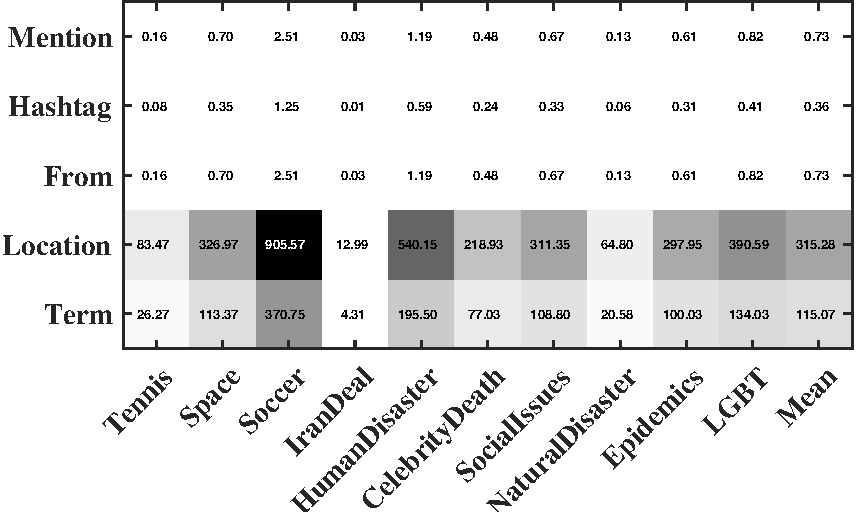
\includegraphics[width=0.5\textwidth]{images/medianMI.pdf}
%\vspace{-3mm}
%\caption{Median MI for different features vs. Topics, last two column show mean value and stderr across all topics}
%\label{fig:medianMI}
%\end{figure}
\begin{figure}[h!]
\centering
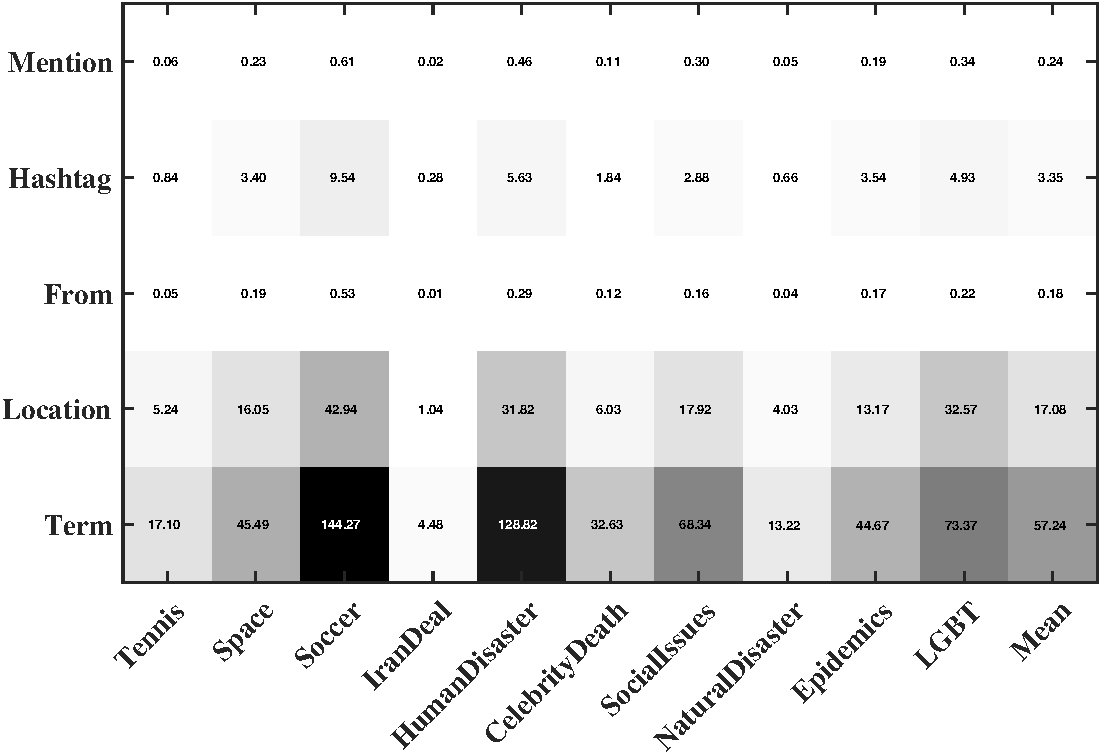
\includegraphics[width=0.5\textwidth, height=60mm]{images/avgMI_gray.pdf}
\vspace{-3mm}
\caption{Mean MI values for different features vs. Topics with the last column as average of mean values across all topics (All values are scaled with $E+10$)}
\label{fig:avgMI}
\end{figure}
%%%%%%%%%%%%%%%%%%%%%%%%%%%%%%%%%%%%%%%%%%%%%%%%%%%%%%%%%%%%%%%%%%%%%%%%%%%

%%%%%%%%%%%%%%%%%%%%%%%%%%%%%%%%%%%%%%%%%%%%%%%%%%%%%%%%%%%%%%%%%%
\begin{table*}[ht]
\centering
{\renewcommand{\arraystretch}{1.2}
\resizebox{\textwidth}{!}{%
\begin{tabular}{|l|l|l|l|l|l|l|l|l|l|l|}
\hline
\textbf{Topics/Top10} & \textbf{NaturalDisaster} & \textbf{Epidemics} & \textbf{IranDeal} & \textbf{SocialIssues} & \textbf{LBGT} & \textbf{HumanDisaster} & \textbf{CelebrityDeath} & \textbf{Space} & \textbf{Tennis} & \textbf{Soccer} \\ \hline
\textbf{From} & earthquake\_wo & changedecopine & mazandara & nsingerdebtpaid & eph4\_15 & ydumozyf & nmandelaquotes & daily\_astrodata & tracktennisnews & losangelessrh \\ \hline
\textbf{From} & earthalerts & drdaveanddee & hhadi119 & debtadvisoruk & mgdauber & syriatweeten & boiknox & freesolarleads & tennis\_result & shoetale \\ \hline
\textbf{From} & seelites & joinmentornetwk & 140iran & debt\_protect & stevendickinson & tintin1957 & jacanews & houston\_\_jobs & i\_roger\_federer & sport\_\_agent \\ \hline
\textbf{From} & globalfloodnews & followebola & setarehgan & negativeequityf & lileensvf1 & sirajsol & ewnreporter & star\_wars\_gifts & tennislessonnow & books\_you\_want \\ \hline
\textbf{From} & gcmcdrought & localnursejobs & akhgarshabaneh & dolphin\_ls & truckerbooman & rt3syria & paulretweet & lenautilus & kamranisbest & makeupbella \\ \hline \hline
\textbf{Hashtag} & earthquake & health & iran & ferguson & tcot & syria & rip & science & wimbledon & lfc \\ \hline
\textbf{Hashtag} & haiyan & uniteblue & irantalks & mikebrown & p2 & gaza & riprobinwilliams & starwars & usopen & worldcup \\ \hline
\textbf{Hashtag} & storm & ebola & rouhani & ericgarner & pjnet & isis & ripcorymonteith & houston & tennis & arsenal \\ \hline
\textbf{Hashtag} & tornado & healthcare & iranian & blacklivesmatter & uniteblue & israel & mandela & sun & nadal & worldcup2014 \\ \hline
\textbf{Hashtag} & prayforthephilippines & depression & no2rouhani & fergusondecision & teaparty & mh370 & nelsonmandela & sxsw & wimbledon2014 & halamadrid \\ \hline \hline
\textbf{Location} & philippines & usa & tehran & st.louis & usa & malaysia & southafrica & germany & london & liverpool \\ \hline
\textbf{Location} & ca & ncusa & u.s.a & mo & bordentown & palestine & johannesburg & roodepoort & uk & manchester \\ \hline
\textbf{Location} & india & garlandtx & nederland & usa & newjersey & syria & capetown & houston & india & london \\ \hline
\textbf{Location} & newdelhi & oh-sandiego & iran & dc & sweethomealabama! & israel & pretoria & austin & pakistan & nigeria \\ \hline
\textbf{Location} & newzealand & washington & globalcitizen & washington & aurora & london & durban & tx & islamabad & india \\ \hline \hline
\textbf{Mention} & oxfamgb & foxtramedia & 4freedominiran & deray & jjauthor & ifalasteen & nelsonmandela & bizarro\_chile & wimbledon & lfc \\ \hline
\textbf{Mention} & weatherchannel & obi\_obadike & iran\_policy & natedrug & 2anow & revolutionsyria & realpaulwalker & nasa & usopen & arsenal \\ \hline
\textbf{Mention} & redcross & who & hassanrouhani & antoniofrench & govchristie & drbasselabuward & robinwilliams & j\_ksen & andy\_murray & realmadriden \\ \hline
\textbf{Mention} & twcbreaking & obadike1 & un & bipartisanism & a5h0ka & mogaza & rememberrobin & jaredleto & serenawilliams & ussoccer \\ \hline
\textbf{Mention} & abc7 & c25kfree & statedept & theanonmessage & barackobama & palestinianism & tweetlikegiris & 30secondstomars & espntennis & mcfc \\ \hline \hline
\textbf{Term} & philippines & health & iran & police & obama & israel & robin & cnblue & murray & madrid \\ \hline
\textbf{Term} & donate & ebola & regime & protesters & gun & gaza & williams & movistar & tennis & goal \\ \hline
\textbf{Term} & typhoon & acrx & nuclear & officer & rights & israeli & nelson & enero & federer & cup \\ \hline
\textbf{Term} & affected & medical & iranian & protest & america & killed & mandela & ΍imperdible & djokovic & manchester \\ \hline
\textbf{Term} & relief & virus & resistance & cops & gop & children & cory & greet & nadal & match \\ \hline
\end{tabular}
}}
\caption{Top 5 features for each topic based on Mutual Information}
\label{table:top10MItopicsLocations}
\end{table*}
%%%%%%%%%%%%%%%%%%%%%%%%%%%%%%%%%%%%%%%%%%%%%%%%%%%%%%%%%%%%%%%%%%
In order to answer the second question on whether any attributes correlate with importance for each feature, we provide two group of analysis. The first group, provides Mutual Information values for each feature across the frequency value of feature attribute shown by violin plots in Fig.~\ref{fig:violinplots}. The attributes for each feature are:

\begin{itemize}
\item \textbf{From}: 
\begin{itemize}
\item favorite count (the number of tweets the user has favorited)
\item followers count (the number of users who follow the user)
\item friends count (the number of users followed by the user)
\item hashtag count (number of hashtags used by the user)
\item tweet count (the number of tweets from the user)
 \end{itemize}
\item \textbf{Hashtag}: tweet count, user count (the number of users using the hashtag)
\item \textbf{Location}: user count
\item \textbf{Mention}: tweet count
\item \textbf{Term}: tweet count
\end{itemize}

As we can see in the violin plots, the general pattern is that the greater the number of tweets, users, or hashtag count a feature has, the greater the chance of becoming topical will be. This pattern exists on other attributes of \textit{From} feature, although the pattern is less visible in comparison with the tweets, users, or hashtag count attributes. 
The second group provides further analysis by plotting density plots of favorite count, follower count, friends count, and hashtag count attributes of \textit{From} feature, demonstrated in Fig.~\ref{fig:densityplots}. Fig.~\ref{fig:densityplots} represents a bi-modality in the distribution of Mutual Information values across attributes dimension. Further analysis of data showed that the top mode belongs to users who have at least one topical tweet while the bottom mode are users with no topical tweets.

%%%%%%%%%%%%%%%%%%%%%%%%%%%%%%%%%%%%%%%%%%%%%%%%%%%%%%%%%%%%%%%%%%%%%%%%%%%
\begin{figure*}[tph!]
\centering
\begin{tabular}{ccccc}
\begin{tabular}{ccccc}
\subfloat[Fig:][]{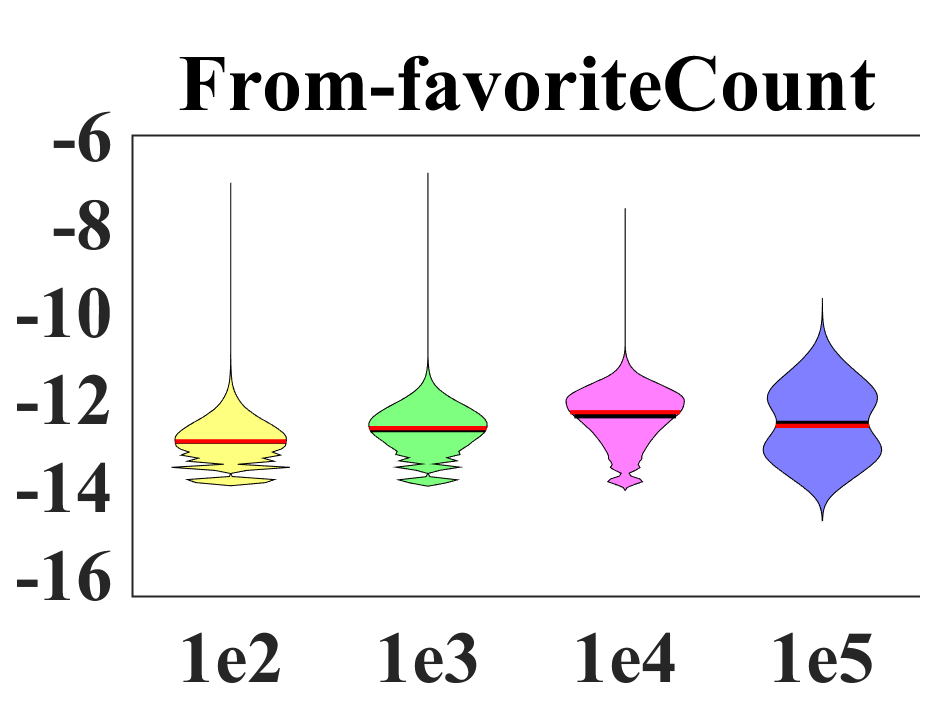
\includegraphics[width=34mm, height=35mm]{images/ViolinPlots/From-favoriteCount.eps}}
\subfloat[Fig:][]{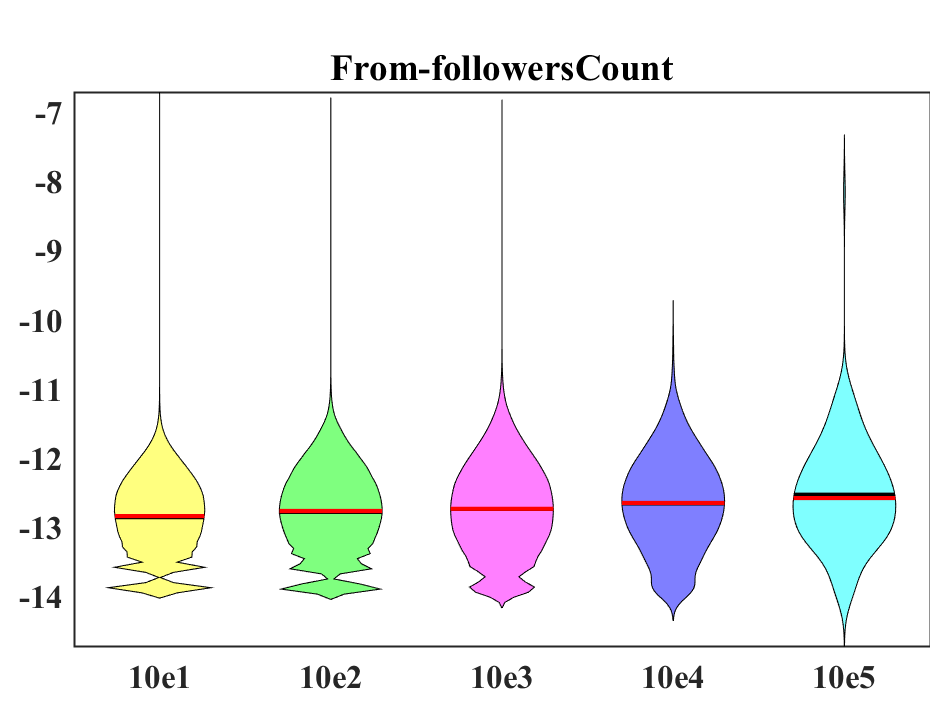
\includegraphics[width=34mm, height=35mm]{images/ViolinPlots/From-followersCount.eps}}
\subfloat[Fig:][]{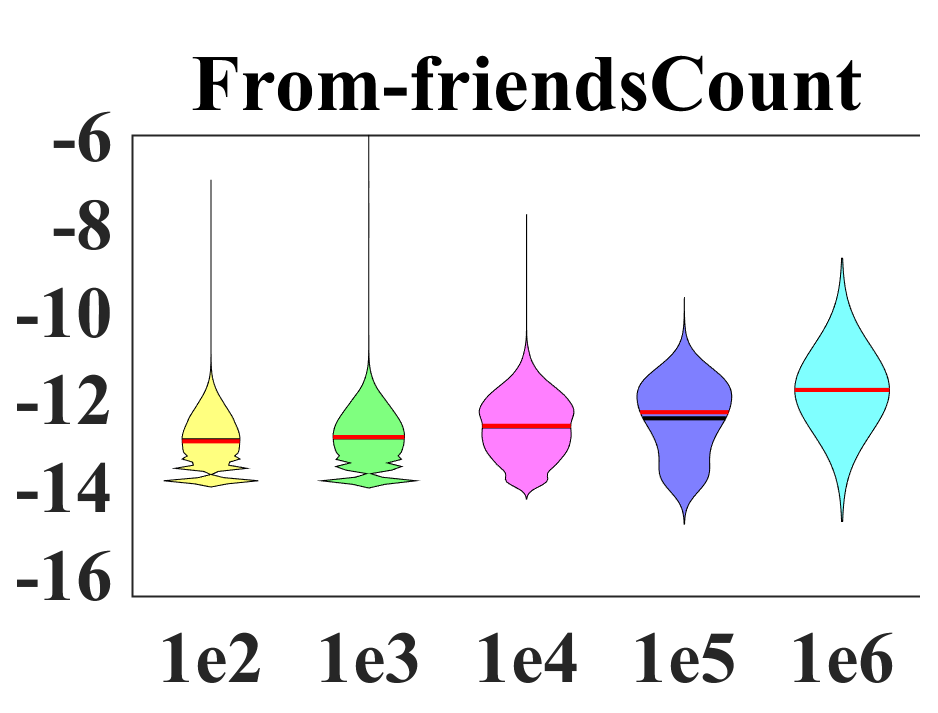
\includegraphics[width=34mm, height=35mm]{images/ViolinPlots/From-friendsCount.eps}}
\subfloat[Fig:][]{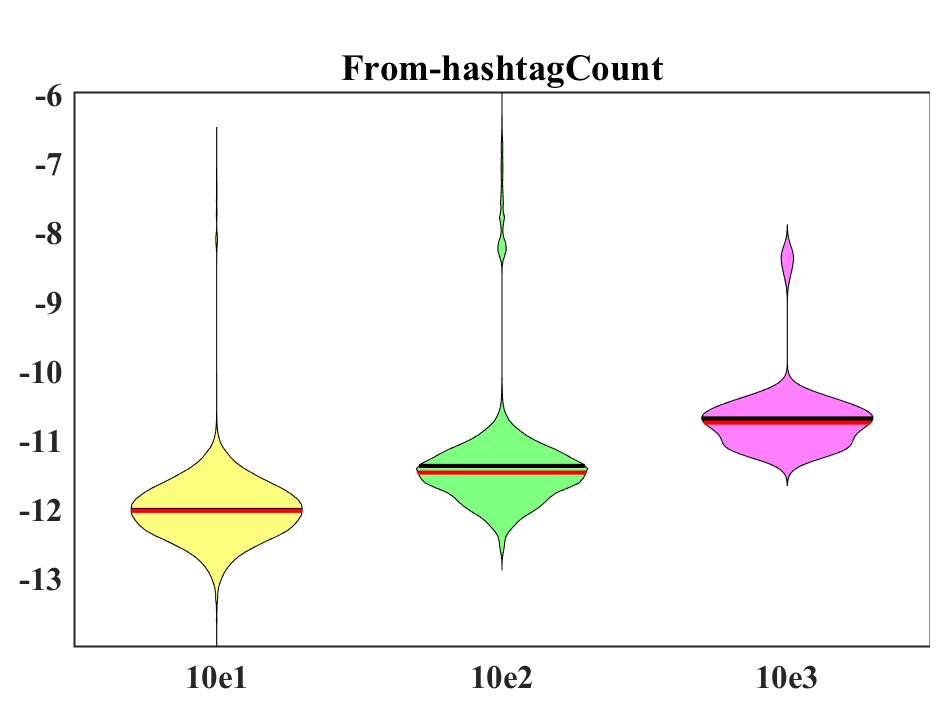
\includegraphics[width=34mm, height=35mm]{images/ViolinPlots/From-hashtagCount.eps}}
\subfloat[Fig:][]{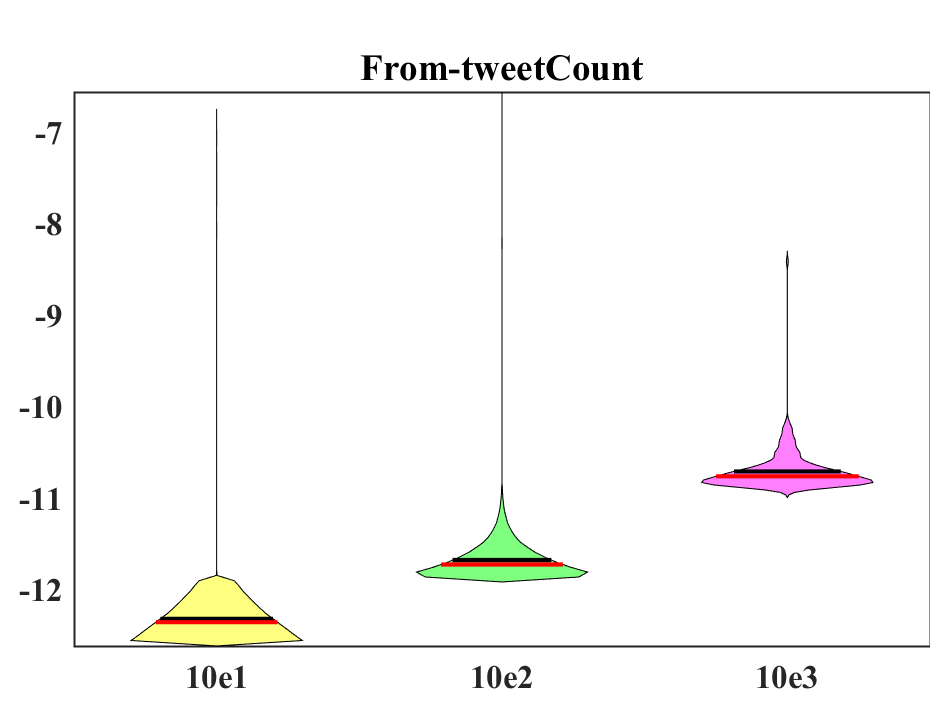
\includegraphics[width=34mm, height=35mm]{images/ViolinPlots/From-tweetCount.eps}} \\
%\vspace{-10mm}
\subfloat[Fig:][]{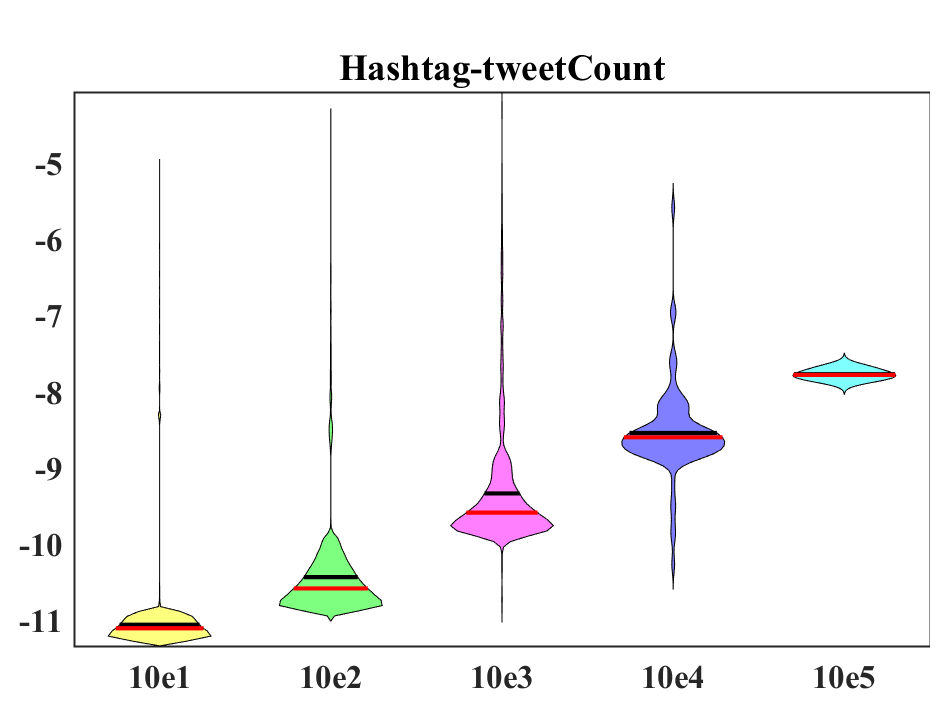
\includegraphics[width=34mm, height=35mm]{images/ViolinPlots/Hashtag-tweetCount.eps}}
\subfloat[Fig:][]{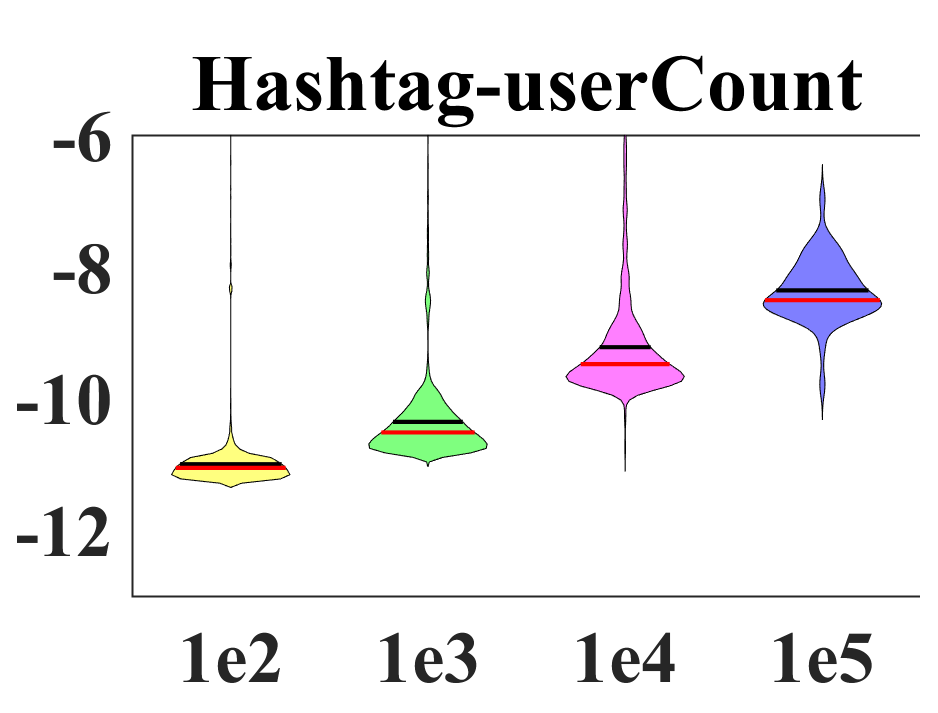
\includegraphics[width=34mm, height=35mm]{images/ViolinPlots/Hashtag-userCount.eps}}
\subfloat[Fig:][]{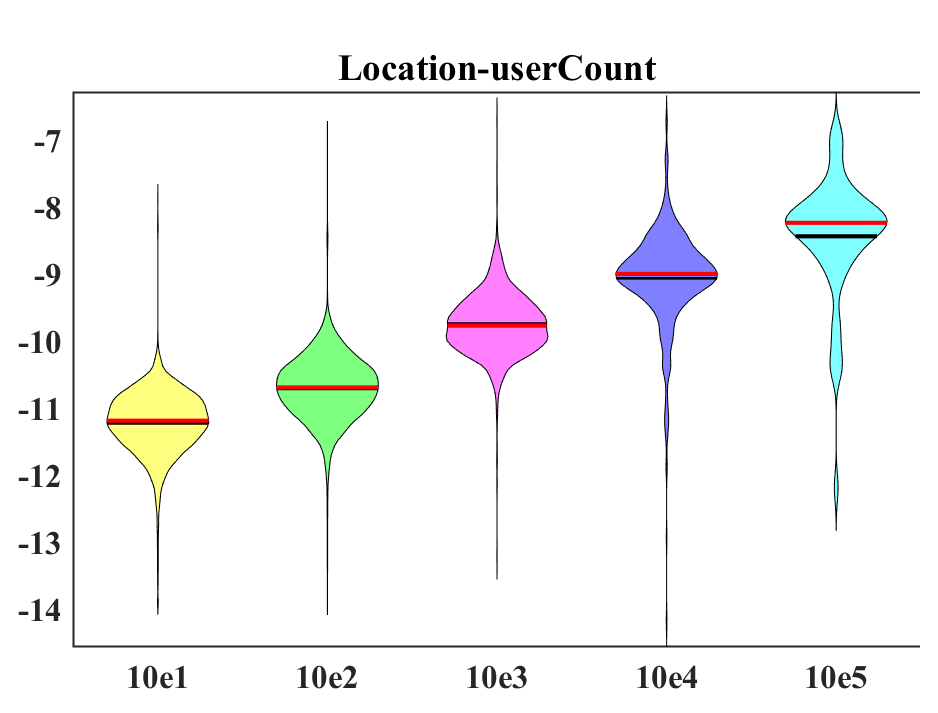
\includegraphics[width=34mm, height=35mm]{images/ViolinPlots/Location-userCount.eps}}
\subfloat[Fig:][]{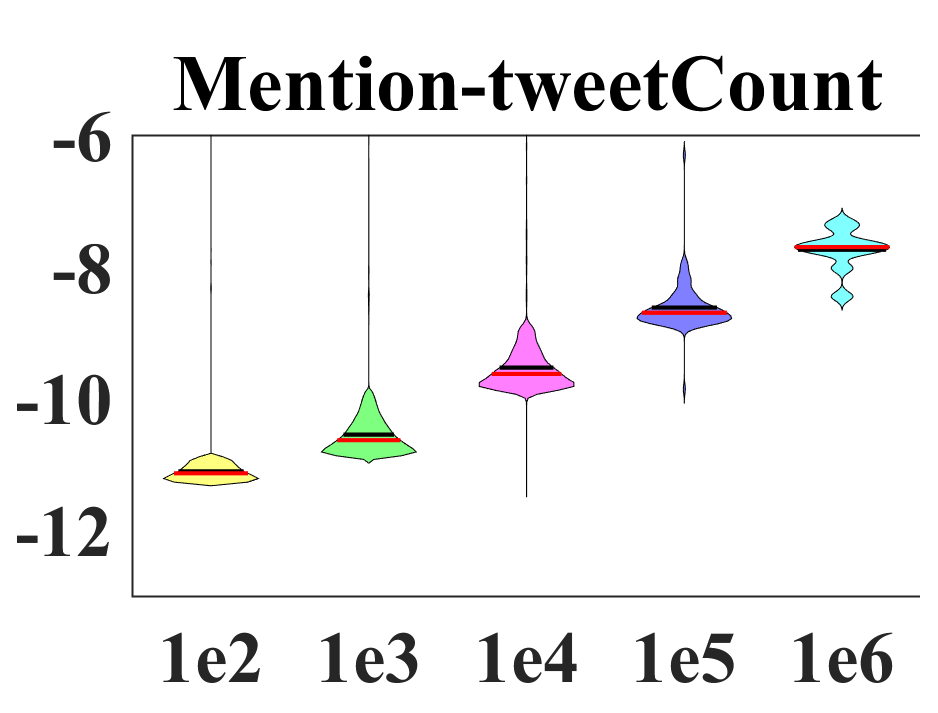
\includegraphics[width=34mm, height=35mm]{images/ViolinPlots/Mention-tweetCount.eps}}
\subfloat[Fig:][]{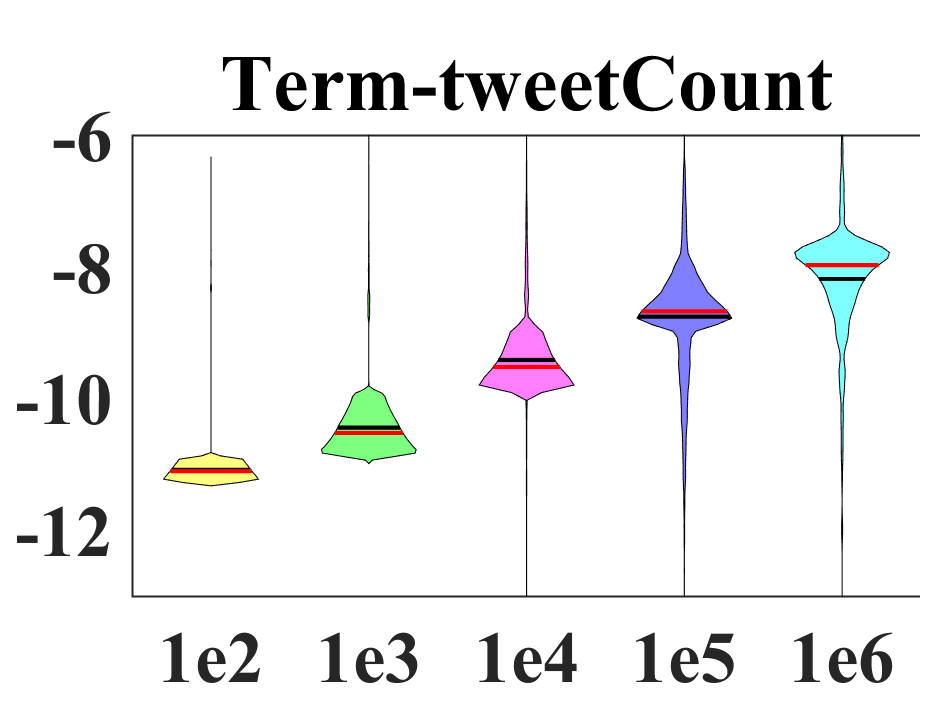
\includegraphics[width=34mm, height=35mm]{images/ViolinPlots/Term-tweetCount.eps}} \\
\end{tabular}
\end{tabular}
\vspace{-2mm}
\caption {ViolinPlots for the frequency values of feature attributes vs. MI. Plots (a-e) respectively show attributes \{favoriteCount, followerCount, friendCount, hashtagCount, tweetCount\} for \textit{From} feature. Plots (f-j) respectively show attributes tweetCount and userCount for \textit{Hashtag}, userCount for \textit{Location} feature, tweetCount for \textit{Mention} and \textit{Term} features.}
\label{fig:violinplots}
\end{figure*}
%%%%%%%%%%%%%%%%%%%%%%%%%%%%%%%%%%%%%%%%%%%%%%%%%%%%%%%%%%%%%%%%%%%%%%%%%%%


%%%%%%%%%%%%%%%%%%%%%%%%%%%%%%%%%%%%%%%%%%%%%%%%%%%%%%%%%%%%%%%%%%%%%%%%%%%
\begin{figure*}[tbh!]
\centering
\begin{tabular}{cccc}
\subfloat[Fig:][]{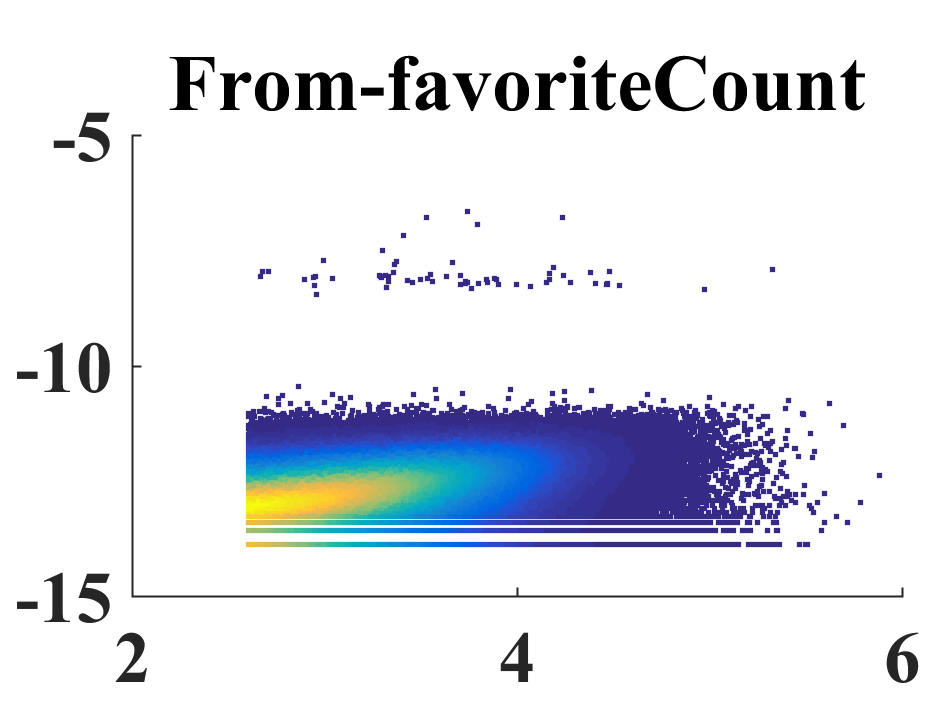
\includegraphics[width=40mm, height=35mm]{images/DensityPlots_IranDeal/dscatterPlot_From-favoriteCount.eps}} \quad
\subfloat[Fig:][]{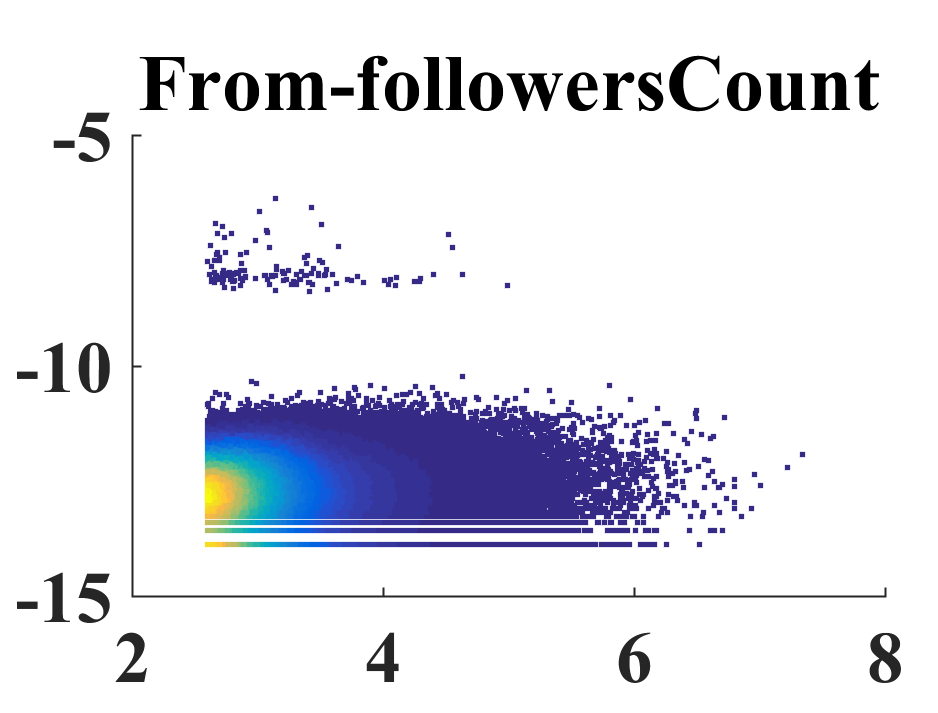
\includegraphics[width=40mm, height=35mm]{images/DensityPlots_IranDeal/dscatterPlot_From-followersCount.eps}} \quad
\subfloat[Fig:][]{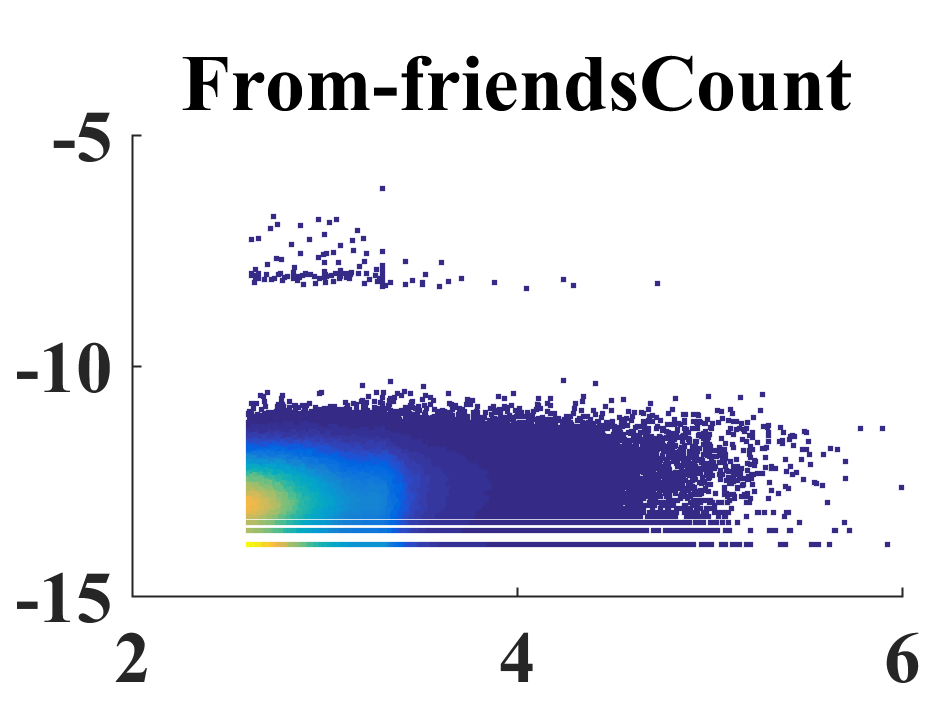
\includegraphics[width=40mm, height=35mm]{images/DensityPlots_IranDeal/dscatterPlot_From-friendsCount.eps}} \quad
\subfloat[Fig:][]{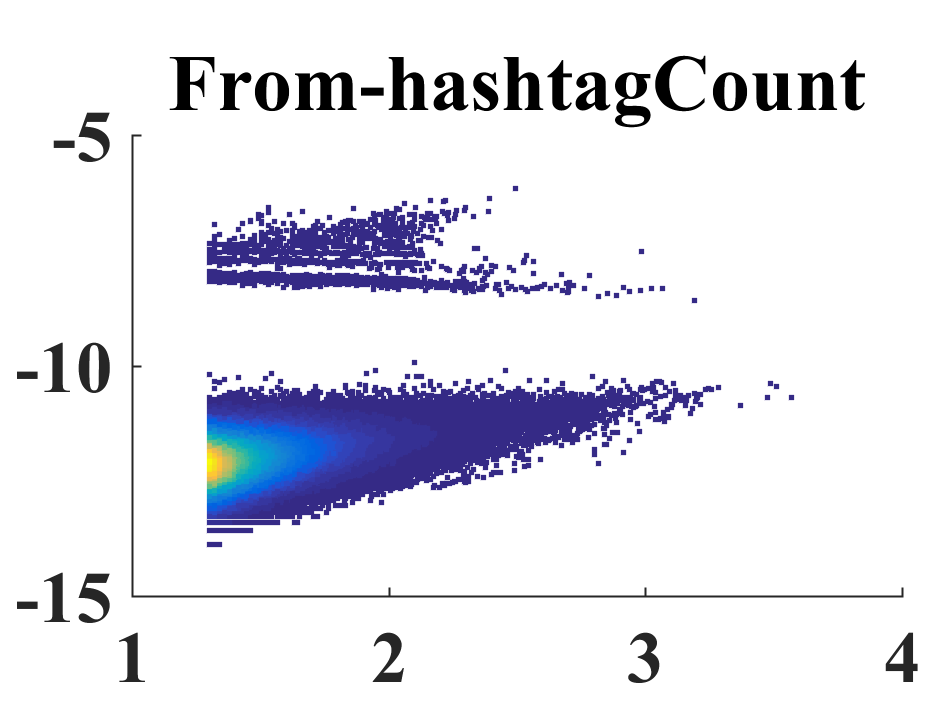
\includegraphics[width=40mm, height=35mm]{images/DensityPlots_IranDeal/dscatterPlot_From-hashtagCount.eps}} \\
\end{tabular}
\vspace{-2mm}
\caption {DensityPlots for the frequency values of feature attributes vs. MI. Plots (a-d) respectively show attributes \{favoriteCount, followerCount, friendCount, hashtagCount\} for \textit{From} feature}
\label{fig:densityplots}
\end{figure*}
%%%%%%%%%%%%%%%%%%%%%%%%%%%%%%%%%%%%%%%%%%%%%%%%%%%%%%%%%%%%%%%%%%